\graphicspath{{Chapters/Theory/Figures/}}
\chapter{Theory}
\label{chap:Theory}

\section{The Standard Model}

The \sm\ of particle physics is a gauge theory describing the
fundamental components of matter and their interactions, and encompasses our
current understanding of the world at particle level. The Standard Model was
formulated in the 1970s, and since then has been tested to an unprecedented
level of precision. %SOME REFERENCES FOR THIS
A brief outline of the \sm\ is given here; it is described in great detail
elsewhere (e.g.~\cite{ALTARELLI:2005zv}).

In the \sm\ there are two main classes of particles: fermions, with half-integer
spin, and bosons, with integer spin. Fermions are the building blocks of matter,
whilst bosons carry the forces of the theory and mediate interactions between the
fermions. The bosons responsible for carrying the fundamental forces all have
spin-1 and are known as \intro{gauge bosons}.
The language of the \sm\ is Quantum Field Theory, and every particle in the \sm\
is associated with a field. The fundamental fermions and the fundamental forces
and their bosons are described in the next two sections, followed by an overview
of electroweak theory.

\subsection{Fundamental Fermions}

There are two types of fermions: quarks and leptons. The quarks are the
constituents of hadrons such as protons and neutrons, whilst the most common
lepton, the electron, is found orbiting the nucleus in the atom. 
The quarks and leptons are arranged into three generations, which each
generation having identical quantum numbers but progressively higher mass. The
different quark and lepton types are referred to as `flavours'. Each
generation of quarks consists of an up-type quark with electric charge
$+$\nicefrac{2}{3}
(named `up', 'charm' and 'top' in the three generations) and a down-type quark
with electric charge $-$\nicefrac{1}{3} (named `down', `strange' and `bottom' in the three
generations); they are shown schematically below

\begin{align}
\left( \begin{array}{c} u \\ d \end{array} \right) \ 
\left( \begin{array}{c} c \\ s \end{array} \right) \ 
\left( \begin{array}{c} t \\ b \end{array} \right) \ 
\end{align}

Each generation of leptons consists of an electrically neutral neutrino
and an electrically charged lepton with charge -1 (the `electron' $e^{-}$, `muon' $\mu^{-}$ and
`tau' $\tau^{-}$); they are shown schematically below

\begin{align}
\left( \begin{array}{c} \nu_{e} \\ e^{-} \end{array} \right) \ 
\left( \begin{array}{c} \nu_{\mu} \\ \mu^{-} \end{array} \right) \ 
\left( \begin{array}{c} \nu_{\tau} \\ \tau^{-} \end{array} \right) \ 
\end{align} 

The neutrinos are assumed to be massless in the \sm, although experimental
evidence suggests that they do in fact have a small mass.

All of the fundamental fermions described above have spin \nicefrac{1}{2}, and they all have an antiparticle partner, with
identical mass but opposite electrical charge\footnote{It is an open question
as to whether or not the neutrino is its own antiparticle.}.
Properties of the fundamental fermions are summarised in~\tab{fundamental-particles}.

\begin{table}[htbp]
\small
\begin{center}
\begin{tabular}{llll} \hline\hline
Particle & Spin & Charge & Mass [GeV] \\ 
\hline
\multicolumn{4}{l}{\bf Gauge Bosons} \\
Photon $\gamma$ & 1 & 0 & 0 \\
Gluon $g$ & 1 & 0 &  0 \\
\Wpm & 1 & $\pm$1 & 80.40 $\pm$ 0.2 \\
\Z & 1 & 0 & 91.188 $\pm$ 0.002 \\
\hline
\multicolumn{4}{l}{\bf Quarks} \\
Up ($u$)        & \nicefrac{1}{2} & $+\nicefrac{2}{3}$ & 1.7-3.3 \timestenpower{-3} \\
Down ($d$)      & \nicefrac{1}{2} & $-\nicefrac{1}{3}$ & 4.1-5.8 \timestenpower{-3} \\
Charm ($c$)     & \nicefrac{1}{2} & $+\nicefrac{2}{3}$ & 1.27 \errAsym{0.07}{0.09}   \\
Strange ($s$)   & \nicefrac{1}{2} & $-\nicefrac{1}{3}$ & 0.10 \errAsym{0.3}{0.2}     \\
Top ($t$)       & \nicefrac{1}{2} & $+\nicefrac{2}{3}$ & 172 \errSym{2} \\
Bottom ($b$)    & \nicefrac{1}{2} & $-\nicefrac{1}{3}$ & 4.2 \errAsym{0.2}{0.1} \\
\hline
\multicolumn{4}{l}{\bf Leptons} \\
Electron ($e^{-}$)              & \nicefrac{1}{2} & -1  & 0.511 \timestenpower{-4} \\
Electron Neutrino ($\nu_{e}$)   & \nicefrac{1}{2} & 0   & $<$ 2\timestenpower{-9} \\
Muon ($\mu^{-}$)                & \nicefrac{1}{2} & -1  & 0.106 \\
Muon Neutrino ($s$)             & \nicefrac{1}{2} & 0   & $<$ 2\timestenpower{-9} \\
Tau ($\tau^{-}$)                & \nicefrac{1}{2} & -1  & 1.7768 \errSym{0.0002} \\
Tau Neutrino ($\nu_{\tau}$)              & \nicefrac{1}{2} & 0   & $<$ 2\timestenpower{-9} \\
\hline
\H & 0 & 0 & \sim 125 \\

\hline\hline
\end{tabular}
\end{center}
\caption{The fundamental particles and their properties~\cite{PDG}.}
\label{table:fundamental-particles}
\end{table} 

\subsection{Fundamental Forces and the Bosons}

At present four fundamental forces are known, and these successfully describe
almost all observed interactions at microscopic levels. They are the
\intro{gravitational force}, the \intro{electromagnetic force}, the \intro{strong force} 
and the \intro{weak force}. 

The gravitational force describes the attraction
between masses. It is by far the
weakest of the known forces (about $10^{38}$ times weaker than the electromagnetic
force), and so has negligible impact on particle interactions. It is
also the only of the four forces not yet formulated in terms of a Quantum Field
Theory and does not enter into the \sm, and so is not discussed any further here.

The electromagnetic force is responsible for interactions between electrically
charged particles, and is responsible for many of the phenomena of the everyday
world, such as the binding of electrons and nuclei into atoms, the binding of
atoms to form more complicated structures and is the source of light. 
It is mediated by the photon ($\gamma$), which couples to
particles carrying electrical charge with a strength given by the particle's
charge and a coupling strength $\alpha=1/137$. The photon has zero
mass, and so electromagnetism is a long range force, and is chargeless so
does not self interact.

The strong force describes interactions between particles carrying a `colour'
charge, and is so called as it is roughly 100 times stronger than the electromagnetic
force. Colour charge is analogous to electrical charge, but comes in three
`types' referred too as red, green and blue, rather than just one as in
the case of electromagnetism. The strong force is mediated by massless gluons. Gluons carry
colour charge, and thus unlike photons can interact with other gluons. This
self-interaction leads to the remarkable property that the strength of the strong force {\it
increases} with distance between two colour charged particles. This in turn leads to {\it
confinement}: bare quarks are never observed in nature, but are only observed
bound together into colour neutral \intro{hadrons} such as protons and neutrons. 
The strong force is also responsible for binding protons and neutrons together
into atomic nuclei.

The weak force is mediated by the \Wpm\ and \Z\ bosons, which couple to particles
carrying weak isospin. It is so named as it is approximately 1000 times weaker
than the electromagnetic force. The \Wpm\ have integer electric
charge, whilst the \Z\ is electrically neutral. Unlike the other gauge bosons
($\gamma,g$), they are both massive and have rather large masses; consequently the weak
interaction is a very short range interaction. The weak force is responsible for
many radioactive decays, the best known of which is beta decay. Uniquely amongst
the known forces, weak interactions allow quarks to change flavour.

Properties of the gauge bosons are summarised in~\tab{fundamental-particles}.

\subsection{The Electroweak Theory}

In the 1960s Weinberg~\cite{PhysRevLett.19.1264} and Salam~\cite{Salam1964168} proposed the unification of the electromagnetic
and weak forces into a single theory which later became known as the
\intro{electroweak} theory. The theory is a gauge theory, guided by requiring that the theory be
invariant under \intro{local gauge transformations}. A gauge theory is a theory
that is invariant under a set of \intro{local transformations}, i.e.
transformations whose parameters have a space-time dependence. Requring
invariance under a local gauge transformation leads the to the emergence of
conserved currents and associated gauge bosons.

The unified \ew\ theory has gauge group

\begin{align}
\uone_{Y} \times \sutwo 
\end{align}

The associated gauge bosons are a massless singlet \Bmu\ associated with the
\uone$_Y$ group and a massless triplet
$\Wmu = \{\Wonemu, \Wtwomu, \Wthreemu\}$ associated with the \sutwo\ group. The $\uone_{Y}$ gauge group is analogous to the
electromagnetic field, but is instead associated with hypercharge Y.

It is observed that weak interactions violate parity conservation; this leads to
different interactions for the \intro{left-handed} and the \intro{right-handed}
components of a particle. A Dirac field, $\psi$, can be expressed as the sum of 
left-handed and right-handed components

\begin{equation}
\psi = \psi_{L} + \psi_{R}
\end{equation}

where

\begin{align}
\psi_{L} = P_{L} = \frac{1}{2} (1 - \gammafive) \psi \\
\psi_{R} = P_{R} = \frac{1}{2} (1 + \gammafive) \psi \\
\end{align}

where $\gammafive$ is the product of the Dirac-gamma matrices $\gammamu$:
$\gammafive = \gamma^{0}\gamma^{1}\gamma^{2}\gamma^{3}$. $P_{L}$ and $P_{R}$
project out the left-handed and right-handed \intro{chiral} states of the
fermion. Chirality is a property of the fermion, but is not a physical
observable. In the limit of massless fermions, the chirality is equal to the
helicity of the particle, i.e. its spin projected onto it's direction of
motion (either +\nicefrac{1}{2} or $-$\nicefrac{1}{2} for a spin \nicefrac{1}{2}
fermion). Experimentally the $W$ boson is seen to only couple to left-handed
chiral states. This is expressed in the theory by arranging the left-handed
particles into \sutwo\ doublets and the right handed particles into \sutwo\
singlets. Considering only the first generation of fermions, we have

\begin{equation}
\lL = \left( \begin{array}{c} \nuL \\ \eL \end{array} \right), \,
\eR, \, \nu_{R}\footnote{The right-handed neutrino does not exist in a model
with massless neutrinos, however given experimental evidence for a small
neutrino mass it is included here for completeness}, \,
\qL = \left( \begin{array}{c} u_{L} \\ d_{L} \end{array} \right), \,
 u_{R}, \, d_{R}
\end{equation}

The \sutwo\ singlets \eR, \nuR, $u_{R}$, $d_{R}$ are invariant under \sutwo\
transformations and thus do not couple to the \Wmu\ gauge bosons, whilst the
doublets transform as

\begin{equation}
\lL \ra \lL' = e^{-iw^{a}\mathbf{T^{a}}}\lL
\end{equation}

where the $\mathbf{T^{a}}$ are the three generators of the \sutwo\ group. These
can be expressed in terms of the Pauli matrices as $\frac{1}{2}
\mathbf{\tau^{a}}$, where

\begin{equation}
\tau^{1} = \left( \begin{array}{cc} 0 & 1 \\ 1 & 0 \end{array} \right), \  
\tau^{2} = \left( \begin{array}{cc} 0 & -i \\ i & 0 \end{array} \right), \  
\tau^{3} = \left( \begin{array}{cc} 1 & 0 \\ 0 & 1 \end{array} \right)
\label{eqn:pauli-matrices}
\end{equation}

The Lagrangian for the massless \ew\ theory is

\begin{align}
\Lagr_{EW}  = & - \frac{1}{4} B_{\mu\nu} B^{\mu\nu} - \frac{1}{4} F^{a}_{\mu\nu}
F^{a\,\mu\nu} \notag \\
& +  i \overline{\lL}^{T} \gammamu \Dmu^{} \lL + i  \overline{\eR}^{T} \gammamu
\Dmu^{} \eR + i \overline{\nuR}^{T} \gammamu \Dmu^{} \nuR \notag \\
& +  i \overline{\qL}^{T} \gammamu \Dmu^{} \qL + i  \overline{u_R}^{T} \gammamu
\Dmu^{} u_R + i \overline{d_R}^{T} \gammamu \Dmu^{} d_{R} 
\label{eqn:ew-lagrangian}
\end{align}

The first line gives kinematic terms for the gauge fields, where $ B_{\mu\nu} =
\partial_{\mu} B_{\nu} - \partial_{\nu} \Bmu$ is the hypercharge field strength,
and  $ F^{a}_{\mu\nu} =
\partial_{\mu} W^{a}_{\nu} - \partial_{\nu} W^{a}_{\mu} - g f^{abc} W^{b}_{\mu}
W^{c}_{\nu}$ is the weak \sutwo\ field strength. The last term in the second
expression gives rise to triple and quartic couplings of the $W^{a}$ bosons.

The second and third lines of Equation~\ref{eqn:ew-lagrangian} describe the
kinematics of the fermions in the theory. The covariant derivative, \Dmu, is
defined such that the quantity \Dmu$\psi$ transforms in the same way as $\psi$
under gauge transforms, and gives rise to interactions between the
fermions and the gauge fields. The covariant derivative operators include the
hypercharge and \sutwo\ operators as needed, and for a fermion multiplet $f$
take the following form

\begin{equation}
\Dmu  =  \partial_{\mu} + i2gI_{W}(f)\mathbf{T^{a}} W_{\mu}^{a} + ig'Y(f)\Bmu
\label{eqn:ew-covariant-derivative}
\end{equation}

%\begin{align}
%\Dmu & =  \partial_{\mu} + ig\mathbf{T^{a}} W_{\mu}^{a} + ig'Y(\lL)\Bmu & \text{for \lL} \\
%\Dmu & =  \partial_{\mu} + ig'Y(\eR)\Bmu & \text{for \eR} \\
%\Dmu & =  \partial_{\mu}  & \text{for $\nu_{R}$} \\
%\Dmu & =  \partial_{\mu} + ig\mathbf{T^{a}} W_{\mu}^{a} + ig'Y(\qL)\Bmu & \text{for \qL} \\
%\Dmu & =  \partial_{\mu} + ig'Y(u_{R})\Bmu & \text{for $u_{R}$} \\
%\Dmu & =  \partial_{\mu} + ig'Y(d_{R})\Bmu & \text{for $d_{R}$} \\
%\end{align}

where $I_{W}(f)$ is the weak isospin and $Y(f)$ is the
hypercharge of fermion $f$ and $g$ and $g'$ are the couplings of the \sutwo\ and
hypercharge fields. The explicit values of $I_{W}$ and $Y$ are as
follows

\begin{gather}
Y(\lL) = - \frac{1}{2},\, Y(\eR) = - 1,\, Y(\nuR) =0,\, Y(\qL) = \frac{1}{6},\, Y(u_{R}) = \frac{2}{3},\, Y(d_{R}) = - \frac{1}{3} \\
I_{W}(\lL) = I_{W}(\qL) = \frac{1}{2}, \  I_{W}(\eR) = I_{W}(\nuR) =  I_{W}(u_{R}) = I_{W}(d_{R}) = 0 
\label{eqn:hypercharges}
\end{gather}

This ensures the desired property that the \sutwo\ field
couples only to the left handed multiplets. 

%that the hypercharge field couples to all
%left and right handed fields except for the neutrino, and 

Substituting Equations~\ref{eqn:ew-covariant-derivative}-\ref{eqn:pauli-matrices}
%, \ref{eqn:hypercharges} and~\ref{eqn:pauli-matrices}
 into~\eqn{ew-lagrangian} gives the following
interaction terms between the leptons and the gauge bosons:

% 5.34 from book
\begin{equation}
\begin{split}
- \frac{g}{2}
\left( \begin{array}{c}\overline{\nu_{L}} \\  \overline{\eL} \end{array} \right)^{T}
%\left( \begin{array}{cc}\overline{\nu_{L}} &  \overline{\eL} \end{array} \right) 
\gammamu \left(
\left( \begin{array}{cc} \Wthreemu & \sqrt{2} \Wpmu \\ \sqrt{2} \Wmmu & -
\Wthreemu \end{array} \right)
- \tan{\thetaW} \Bmu \right)
\left( \begin{array}{c} \nu_{L} \\  \eL \end{array} \right) \\
+ g \tan{\thetaW} \, \overline{\eR} \, \gammamu \Bmu \eR
\end{split}
\label{eqn:ew-lepton-interactions}
\end{equation}

where the $W^{1}, W^{2}$ have been rewritten as $W^{\pm} = (W^{1} \mp
iW^{2})/\sqrt{2}$, and \thetaW\ is the weak mixing angle, defined such that

\begin{equation}
g \sin{\thetaW} = g' \cos{\thetaW}
\end{equation}

In~\eqn{ew-lepton-interactions} four gauge bosons are seen: a charged \Wp\ and
\Wm\ which mediate transitions between electrons and neutrinos, and a neutral
\Wthreemu\ and \Bmu\ which both couple to pairs of electrons and neutrinos.
These can not be identified with the physical \Z\ boson and photon, since the
photon does not couple to the neutrino.  However, the physical bosons can be obtained by replacing the fields \Wthreemu\ and \Bmu\ by the
physical particles \Zmu\ and \Amu

\begin{align}
\Zmu & = \cos{\thetaW} \Wthreemu - \sin{\thetaW} \Bmu \\
\Amu & = \cos{\thetaW} \Bmu + \sin{\thetaW} \Bmu
\end{align}

Substituting these into~\eqn{ew-lepton-interactions} and collecting terms
relating to each of the gauge bosons, it is found that the
charged \Wpm\ bosons mediate transitions between left-handed electrons and
neutrinos with the term

\begin{equation}
- \frac{g}{2\sqrt{2}} \left( \overline{\nuL} \gammamu \eL \Wpmu
\ + \  \overline{\eL} \gammamu \nuL \Wmmu \right)
\end{equation}

The photon couples equally to left- and right-handed electrons, but not to the
neutrinos

\begin{equation}
g \sin{\thetaW} \left( \overline{\eL} \gammamu \eL 
\ + \ \overline{\eR} \gammamu \eR \right) \Amu
 = g \sin{\thetaW} \, \overline{e}\, \gammamu e \Amu
\end{equation}

The quantity $g \sin{\thetaW}$ can thus be associated with the electromagnetic
charge $e$. The \Z\ boson couples to left- and right-handed electrons and to
neutrinos, with slightly different couplings to the left- and right-handed
electrons

\begin{equation}
\frac{g}{2 \cos{\thetaW}} \left( 
(1 - 2 \sin^{2}{\thetaW})\, \overline{\eL} \gammamu \eL  - 2 \sin^{2}{\thetaW}\, \overline{\eR} \gammamu \eR 
- \overline{\nuL} \gammamu \nuL 
\right)\Zmu
\end{equation}

Thus the \W\ and \Z\ bosons are associated with the weak force, and the photon
to the electromagnetic force. Similarly it is found that the \W\ boson mediates
transitions between left-handed $u$ and $d$ quarks, that the photon couples to
quarks with couplings proportional to their electric charge, and that the
\Z\ boson couples to quarks proportionally to their weak isospin and electric
charge, with different couplings for the different chiral states.

Generally, the covariant derivative of~\eqn{ew-covariant-derivative} can be
written in terms of the physical fields \Wpmmu, \Zmu, \Amu\ as

\begin{equation}
\Dmu  =  \partial_{\mu} + i \frac{g}{\sqrt{2}} ( \Wpmu + \Wmmu ) 
+ i \frac{g}{\cos{\thetaW}} ( I^{f}_{3} - Q^{f} \sin^{2}{\thetaW} ) \Zmu
+ i g Q^{f} \sin{\thetaW} \Amu
\label{eqn:ew-covariant-derivative-full}
\end{equation}

for a fermion $f$ possessing a third component of weak isospin $I_{3}^{f}$
and an electromagnetic charge $Q^{f}$. The electromagnetic charge can be related
to the hypercharge as $Q = I_{3} + Y$. The second term
in~(\ref{eqn:ew-covariant-derivative-full}) describes the weak Charge Current (CC)
interaction, the third the weak Neutral Current (NC) and the fourth the
electromagnetic neutral current.

\subsection{Electroweak Symmetry breaking}

The gauge bosons and fermions in the \ew\ Lagrangian given
in~\eqn{ew-lagrangian} are massless. This is clearly a problem as the fermions
are observed to be massive, and more worryingly the $W$ and \Z\ bosons are
observed to be extremely massive. Unfortunately, it is not possible to formulate a locally gauge invariant theory with massive
gauge bosons, and it is not possible to include explicit mass terms for the
fermions as this mixes the left- and right-handed fermions, which have been
assigned to different \sutwo\ multiplets. 

In order to give
mass to the gauge bosons, the symmetry must be broken somehow. The simplest way
to do so would be to simply add mass terms for the gauge bosons by hand, however
this would lead to a non-renormalisable theory which would contain an infinite
number of divergences. Instead, gauge bosons are given masses by `spontaneous
symmetry breaking' in the Higgs mechanism\footnote{more properly the Brout-Englert-Higgs
mechanism} by introducing an \sutwo\ doublet of complex scalar fields (the \intro{Higgs
Field}), with a potential of the form:

\begin{equation}
%\Lagr_{H} = (\partial_{\mu} \Phi)(\partial^{\mu} \Phi) - {\mu}
V(\Phi) =  \mu^{2}\Phi^{\dagger}\Phi + \lambda(\Phi^{\dagger}\Phi)^{2}
\end{equation}

If $\mu^{2} < 0$ then the field has a minimum at $\Phi^{\dagger}\Phi = -
\frac{1}{2} \mu^{2}/\lambda$, and thus has a non-zero vacuum expectation value. 
Gauge invariance of the lagrangian is preserved, however the vacuum state is no
longer invariant under gauge transformations.
The gauge bosons acquire mass by interactions with the field, and it is found
that

\begin{equation}
M_{W} = \frac{1}{2}gv, \ M_{Z} = \frac{gv}{\cos{\thetaW}}
\end{equation}

where $v = \mu / \sqrt{\lambda}$. 

Terms can also be
introduced describing interactions of the fermions with this field, giving
masses to the fermions without mixing the left- and right-handed components.
Such an interaction is called the `Yukawa interaction'. The couplings strengths
are given by the \intro{Yukawa couplings}, which can be different for each
fermion and are not fixed by the theory, requiring experimental determination. 

The introduction of the Higgs field predicts the existence of one further
fundamental particle, a massive scalar boson known as the \intro{Higgs Boson},
with mass $m_{H} = \sqrt{2}\mu$. Again, the mass is not predicted by the theory. 
There has
been much experimental activity in the search for the Higgs boson, and for many
years it proved elusive. Recently,
the CMS~\cite{CMS_Higgs:2012gu} and ATLAS~\cite{ATLAS_Higgs:2012gk} collaborations reported evidence for a new boson with
properties consistent with the Higgs.

\section{Interactions in proton-proton collisions}
\label{sec:Theory-ppInteractions}

A sketch of a proton-proton collision at a hadron collider is shown in
\fig{pp-event}. In proton-proton collisions it is not the
protons themselves that interact but their quark and gluon constituents.
In a basic picture, the proton consists of three \intro{valence quarks}:
two up-quarks and one down-quark, bound together by the strong force. These
quarks will spontaneously exchange gluons, which can in turn split into
additional quark pairs, known as \intro{sea quarks}. As the energy of a
particle used to probe the proton is increased, the fraction of the proton
momentum observed to be carried by the sea quarks and gluons increases, as one
is able to resolve the structure of the proton at a finer level. The content of
the proton thus depends on the momentum transfer of the interaction $Q^{2}$.
Perturbative QCD breaks down at these small scales, and the structure of the
proton must thus be described by fits to experimental data. \intro{Parton Density Functions
(\partDF s)} are used to describe the probability of finding a parton of flavour $i$ carrying a
fraction $x_i$ of the incoming proton momentum at a momentum scale $Q^{2}$.

The interaction between two \intro{incoming} partons (quarks or gluons) from the two initial
protons is known as the \intro{hard scatter}, which will lead to two or more
hard outgoing particles. The incoming and any coloured outgoing particles will
emit further further QCD radiation known as \intro{initial state radiation (ISR)} 
and \intro{final state radiation (FSR)} in the form of gluons, which in turn can
split into further partons. Once the outgoing quarks and gluons become far enough from
one other, the coupling between them becomes strong and they form into colour neutral
hadrons in a process known as hadronisation. Charged incoming and outgoing
particles will also emit QED radiation in the form of photons. 

The interaction between the incoming
particles leaves behind other partons from the breakup of the original proton.
There may also be other secondary collisions between these residual partons,
referred to as \intro{multiple interactions}. Particles from ISR and FSR, the breakup of the proton and
multiple interactions are collectively referred to as the \intro{Underlying Event
(UE)}.

\begin{figure}
\centering
        \vspace{-5mm}
    \subfigure[]{
        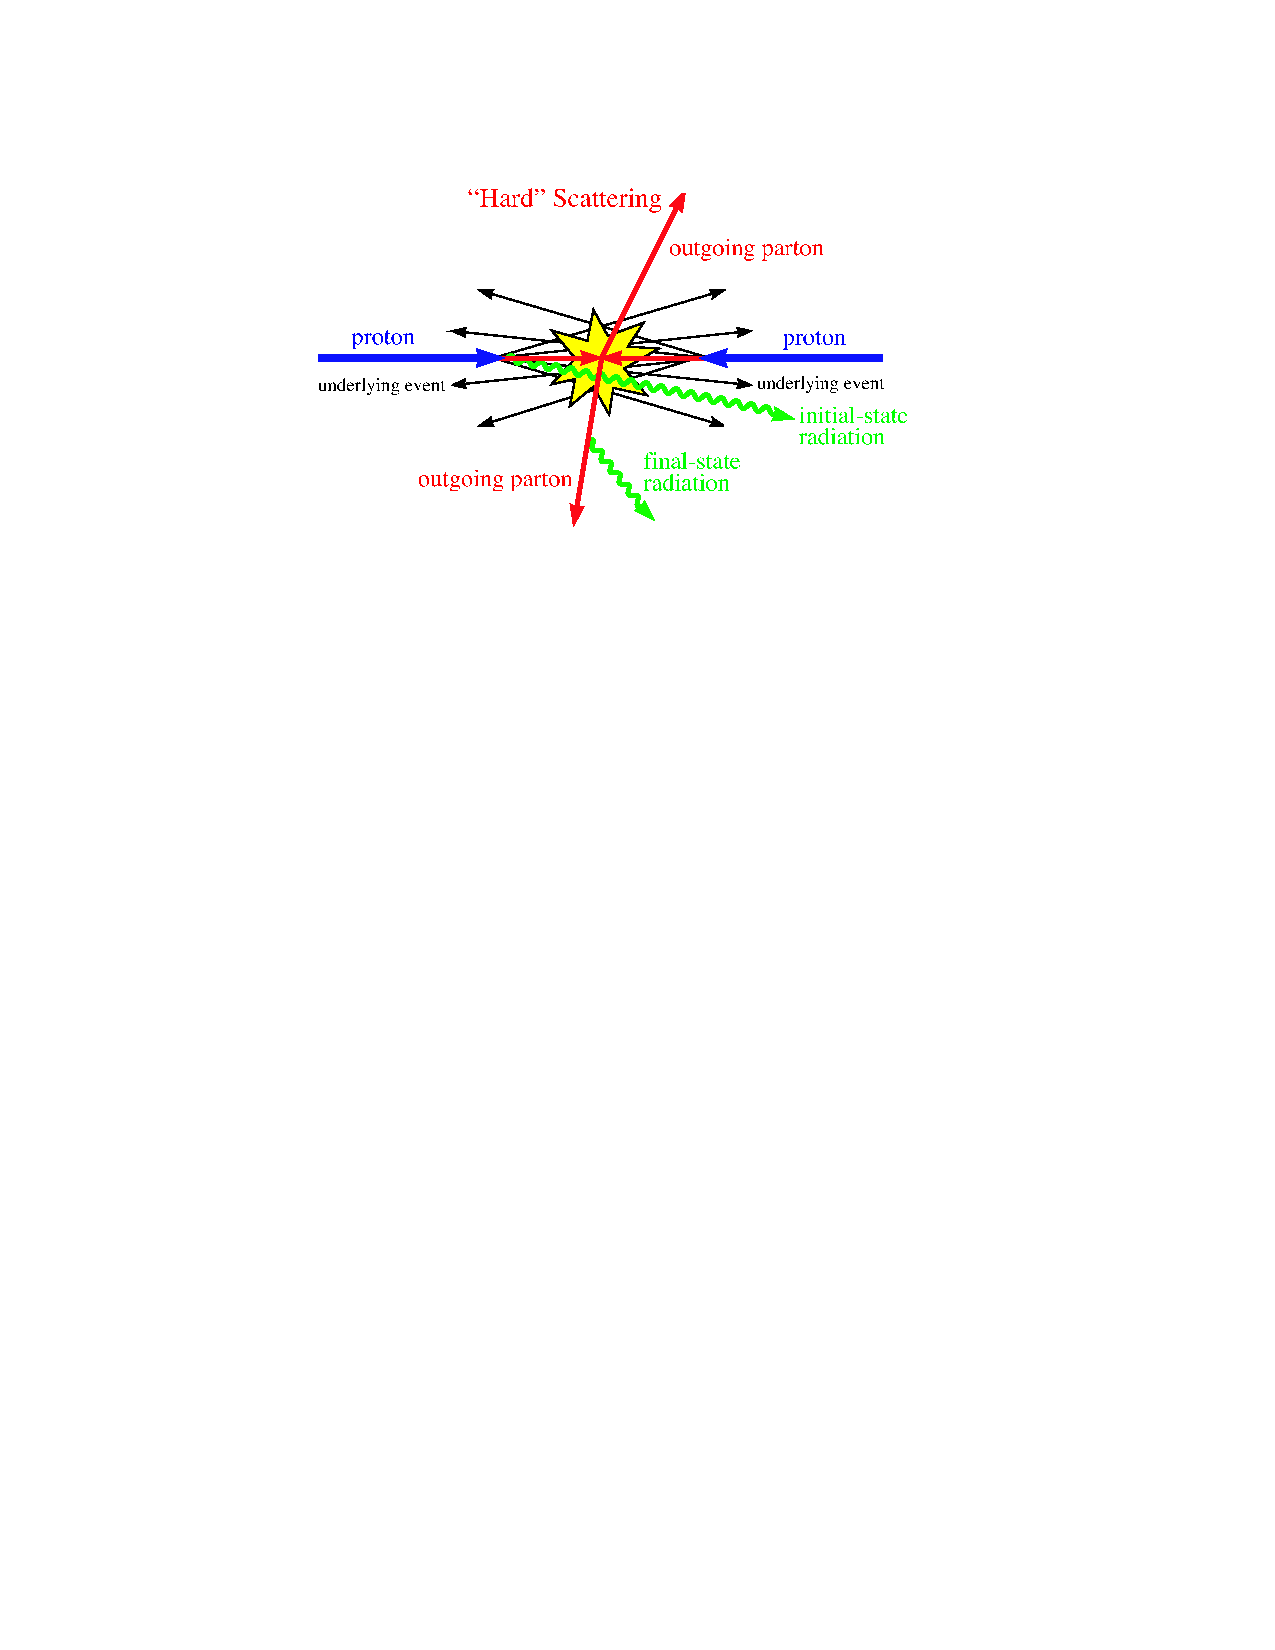
\includegraphics[width=0.47\textwidth]{pp_event}
    }
    \caption{\small
Sketch of a proton-proton collision. Figure from~\cite{Campbell:2006wx}.
}
    \label{fig:pp-event}
\end{figure}

\section{Monte-Carlo Simulation}
\label{sec:Theory-MC}

Simulated events are a crucial ingredient to a particle physics
measurement for a number of reasons. It is of course important to be able to
compare experimentally measured quantities such as \cx s and kinematic
distributions with predictions from the theory. Furthermore, simulated data
samples are important for calibrating the detector response and for estimating
selection efficiencies in order to translate from observed events
to a physical quantity such as a \cx. 

Simulated events are obtained by
means of \mc\ simulations, which use numerical integration to calculate matrix
elements and generate events. Generating events suitable for the purposes
outlined in the last paragraph typically consists of four steps:
calculation of the matrix element for the hard scattering, adding additional and
final state radiation using a parton shower,
hadronisation and finally embedding in the underlying event. These steps are described
in more details below. 

The calculation of the matrix element (ME) is
made at a fixed order in perturbative QFT, where the expansion is in terms of
the strong coupling constant \alphaS. The event generators used in this thesis
are either \intro{Leading Order (LO)}, where only the simplest diagrams
contributing to a process are calculated, or \intro{Next to Leading Order (NLO)},
where contributions from one loop diagrams are included. 

Both the incoming and any outgoing quarks and gluons
(collectively, partons) will emit soft collinear radiation in the form of other quarks and gluons. This is
modelled by the parton shower (PS), which in the case of outgoing partons
successively radiates the partons until they reach an energy of $\sim 1$ \gev, at
which point the predictions of perturbative QCD become invalid and the partons
hadronise. The process of hadronisation is not well described theoretically,
but relies on a number of phenomenological models. In \intro{string models} the
force between two coloured charges is modelled as an elastic string with
rising tension as the particles separate. If the string is stretched too much
it will snap, creating a new pair of colour charges. If a pair of opposite
colour charges are found close to each other they are combined into a hadron.

For the incoming partons, the
shower is run in-reverse back to the \intro{factorisation scale, \uF}, at which
point the calculation is connected to the \partDF. The
factorisation scale thus sets the boundary between hard, perturbative QCD and
soft, non-perturbative QCD.  

Modern \mc\ integrators can calculate exact matrix elements with additional
partons from FSR in the matrix element. Whilst this increases the accuracy of
the \cx\ and kinematic distributions, it becomes necessary to `match' the
ME calculation to the PS, to ensure no double counting (since otherwise a
$2\ra3$ event could either come from a $2\ra3$ matrix-element event or a $2\ra2$
matrix element event with an additional parton coming from a splitting in the
parton shower. Different generators use different models for the parton
shower, hadronisation, and the ME-PS matching.

A second scale involved in the generation of events is the
\intro{renormalisation scale, \uR}. Since gluons are massless, QCD contains UV
divergences which lead to infinite results in cross-section calculations. Since 
this is clearly unphysical, a renormalisation procedure is used to cancel the
divergences, for example by introducing a gluon mass or setting a UV cutoff
scale to regularise the divergence. The divergences are then absorbed by a
redefinition of the `bare' parameters of the theory to the physically observable
parameters. Renormalised parameters such as \alphaS\ are thus dependant on \uR.
When performing calculations to all orders of perturbation theory,  the results
should not depend on the choice of \uR\ or of \uF\ - however since in LO and NLO
calculations the expansion is truncated after the
first few terms,  the results will heavily depend on
the choice of \uR\ and \uF. Calculations performed at NLO are expected to
be less dependant on the choice of scale than LO calculations, however
theoretical uncertainties must be assigned to account for the dependence on the
(somewhat arbitrary) choice of scale. Typically this is done by setting the
scales to an energy similar to the momentum transfer in the interaction, then
varying up and down by a factor of two to estimate systematics.

\subsection{\mc\ generators}
\label{sec:Theory-MC-gen}

A wide range of \mc\ integrators and event generators are available to simulate
processes of interest at the LHC. The
following generators are used in this thesis. For each generator, an outline of
how it is used and its general properties is given.

\begin{itemize}
    \item \mcfm ~\cite{Campbell:2011} is designed to calculate \cx s for
    femtobarn-level processes at hadron colliders. Matrix elements are
    calculated at NLO, incorporating full spin correlations. \mcfm\ is a \cx\
    calculator only and cannot produce unweighted events suitable for use in a
    physics analysis. Nevertheless it provides a useful toolkit for calculating
    \cx s, estimating the acceptance of the fiducial volume and studying the
    associated uncertainties due to \partDF\ and scale uncertainties.

    \item \powhegbox~\cite{Alioli:2010xd} is a general framework for implementing
    NLO calculations. It uses the \powheg\ method to match the NLO matrix
    elements to the parton shower. \powhegbox\ must be interfaced to an external
    program for the implementation of the parton shower - in this thesis
    \powhegbox\ is interfaced to \pythia for showering. Specific details of the
    implementation of the \ZZ\ process in \powhegbox\ is given
    in~\cite{Melia:2011tj}; the \ggZZ\ process is not included. 
    Samples generated using \powhegbox\ are used as the main signal samples for
    the \qqZZ\ process, used to optimise the selection, estimate selection
    acceptances and systematics and compare observed distributions with theory.

    \item \ggtwoZZ~\cite{gg2ZZ} is a specialist generator used to simulate the
    \ggZZ\ process. Events generated with \ggtwoZZ\ are used in conjunction with
    the \powhegbox\ events as the main signal sample. It is interfaced to the
    \herwig\ to provide the parton shower and \jimmy~\cite{bib:jimmy} to model the underlying
    event. Its sister generator, \ggtwoWW, is used to simulate the background
    from \ggWW~\cite{Binoth:2006mf}.

    \item \sherpa~\cite{Gleisberg:2008ta} is a LO generator, capable of
    simulating the \qqZZ\ process with up to three additional hard partons in the matrix element. It
    uses an extended version of the CKKW scheme~\cite{Hoeche:2009rj} to match to the matrix element to the parton shower,
    and provides its own simulation of the parton shower, QED radiation and
    the underlying event. \sherpa\ is also capable of simulating aTGCs. It is
    used as a cross-check to \powhegbox\ and to estimate the impact
    of uncertainties
    arising from different implementations of the parton shower and QED
    radiation. It is also used to simulate aTGC samples.
    Version 1.3.1 is used to simulate \qqZZllll\ at 7 \tev, and 1.4.0 is used at
    8 \tev.

    \item \pythia is a LO generator which uses a library of $2\ra2$
    matrix elements covering almost all \sm\ processes to model the signal
    process and a \pt\ ordered parton shower to model additional radiation.
    The Fortran77 based
    \pythia6~\cite{pythia} is used at 7 \tev\, whilst the C++ based
    \pythia8~\cite{Sjostrand:2007gs} is used at 8 \tev. \pythia is used to
    provide showering for many of the other generators described here, and is
    also used as a cross-check to the main signal samples.

    \item \herwig~\cite{Herwig} is another general purpose LO generator, generating events in a
    similar way is used to \pythia, but using an angular-ordered parton shower.
    %and cluster model for hadronisation.
    It is used for generating inclusive samples (all final
    states) of $WW$ and $WZ$ production, used in estimating background from
    other diboson processes.

    \item \herwigPP~\cite{Bahr:2008pv} is a C++ based generator based on the
    Fortran \herwig. It includes NLO calculations of a number of processes
    using the \powheg\ matching scheme. \herwigPP\ is only used for comparison
    of \ZZ\ event kinematics at generator level.

    \item \mcatnlo~\cite{bib:mcatnlo} is a NLO generator, and was the first
    generator to implement NLO ME to PS matching, using the so-called \mcatnlo\
    technique. \mcatnlo\ is used to simulate the background processes \ttbar,
    \Wt\ and single-top at 7 \tev. \mcatnlo\ can simulate \qqZZ, but only in the
    zero-width approximation where the lineshape of the \Z\ boson is not
    included. For this reason \mcatnlo\ is not used for signal simulation,
    though the generator level predictions of \mcatnlo\ are compared to other
    generators in the following section.

    \item \alpgen~\cite{alpgen} is a LO genertor for simulating multi-parton
    processes in hadron interactions. It can simulate $W$ and \Z\ production
    with up to 6 additional partons in the matrix element. It is interfaced to
    \herwig\ for the parton shower, using the MLM matching
    scheme~\cite{Mangano2002343}. It is used to simulate \W\ and \Z\ bosons in
    association with jets, as well as low mass Drell-Yan and \Wg and \Zg.

    %\item \pythiaB is used to simulate events with heavy favour dijets. Since
    %these are of interest as background processes to events with leptons, a
    %dilepton filter is applied at generator level, requiring two $e$ or $\mu$ with
    %\ptgt{10}.

    %\item \madgraph~\cite{madgraph} \Wg\ and \Zg (7 tev).

\end{itemize}

